\documentclass[landscape]{article}

\usepackage[utf8]{inputenc}
\usepackage[english]{babel}

\usepackage{amsmath,amsfonts,amssymb}
\usepackage{fullpage}
\usepackage{verbatim}

\usepackage{tikz,pgfplots}

\pgfplotsset{
    width=160mm,height=150mm,
    major grid style={thin,dotted,color=black!50},
    minor grid style={thin,dotted,color=black!50},
    grid,
    every axis/.append style={
        line width=0.5pt,
        tick style={
            line cap=round,
            thin,
            major tick length=4pt,
            minor tick length=2pt,
        },
    },
    legend cell align=left,
    legend pos=north west,
}

%%%%%%%%%%%%%%%%%%%%%%%%%%%%%%%%%%%%%%%%%%%%%%%%%%%%%%%%%%%%%%%%%%%%%%%%%%%%%%%%

\begin{document}

\section{Strong-Scaling (200MB)}
% IMPORT-DATA stats result/result_algorithm.txt

\begin{center}
    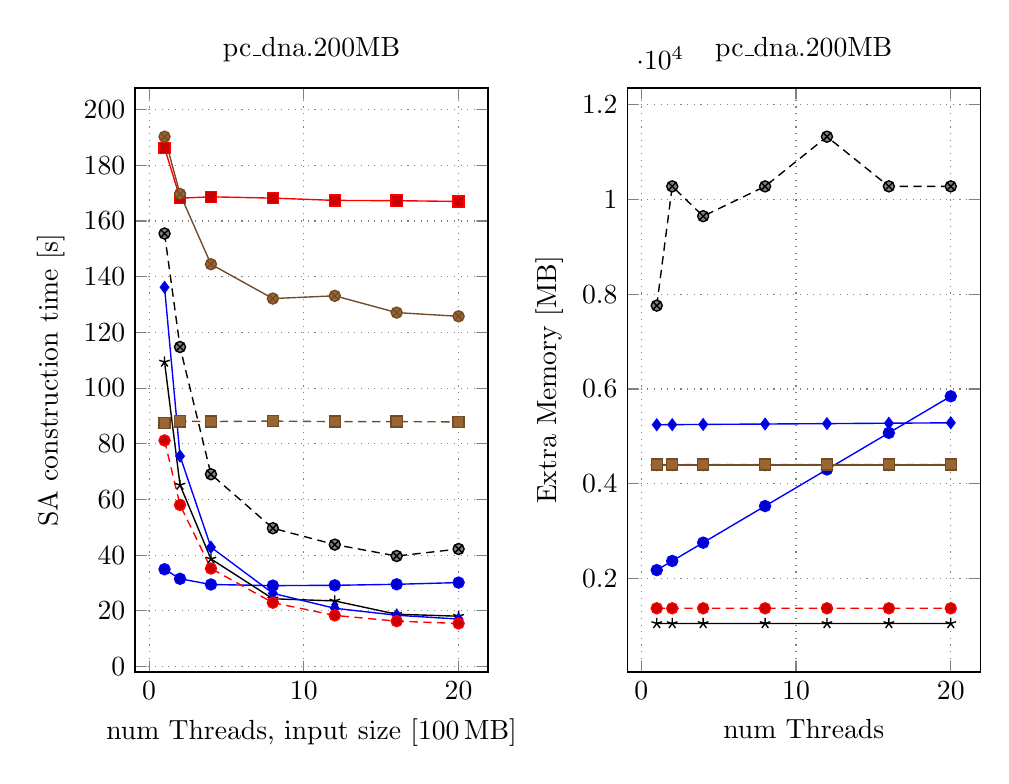
\begin{tikzpicture}
        \begin{axis}[
                name=axis1,
                width=0.5\textwidth,
                height=90mm,
                title={pc\_dna.200MB},
                xlabel={num Threads, input size [100\,MB]},
                ylabel={SA construction time [s]},
                legend columns=4,
                legend to name=legend0,
                legend style={
                    /tikz/every even column/.append style={column sep=0.5cm,black},
                    /tikz/every even column/.append style={black},
                },
            ]

            %% MULTIPLOT(algo) SELECT thread_count AS x, time/1000 AS y, MULTIPLOT
            %% FROM stats WHERE rep_id=1 AND input="pc_dna.200MB" GROUP BY MULTIPLOT,x ORDER BY MULTIPLOT,x
            \addplot coordinates { (1,34.9109) (2,31.4859) (4,29.4439) (8,29.0382) (12,29.1495) (16,29.5131) (20,30.1302) };
            \addlegendentry{algo=BPR\_par};
            \addplot coordinates { (1,186.307) (2,168.193) (4,168.687) (8,168.221) (12,167.406) (16,167.3) (20,167.024) };
            \addlegendentry{algo=DC3-Parallel-2};
            \addplot coordinates { (1,190.286) (2,169.704) (4,144.477) (8,132.142) (12,133.129) (16,127.104) (20,125.769) };
            \addlegendentry{algo=DC3\_parallel};
            \addplot coordinates { (1,109.363) (2,65.1653) (4,38.6184) (8,24.3101) (12,23.5421) (16,18.7592) (20,18.05) };
            \addlegendentry{algo=Deep-Shallow\_par};
            \addplot coordinates { (1,136.202) (2,75.5735) (4,42.832) (8,26.2677) (12,20.8961) (16,18.3966) (20,17.018) };
            \addlegendentry{algo=Discarding4Parallel};
            \addplot coordinates { (1,81.1837) (2,58.0266) (4,35.1818) (8,22.9087) (12,18.3419) (16,16.2675) (20,15.4456) };
            \addlegendentry{algo=DivSufSort\_PARALLEL\_ref};
            \addplot coordinates { (1,87.5125) (2,88.052) (4,87.9809) (8,88.1244) (12,87.9322) (16,87.9396) (20,87.8446) };
            \addlegendentry{algo=GSACA\_parallel};
            \addplot coordinates { (1,155.504) (2,114.74) (4,69.0391) (8,49.6525) (12,43.7744) (16,39.6675) (20,42.1922) };
            \addlegendentry{algo=Osipov\_parallel\_wp};

        \end{axis}
        \begin{axis}[
                at={(axis1.outer north east)},
                anchor=outer north west,
                name=axis2,
                width=0.5\textwidth,
                height=90mm,
                title={pc\_dna.200MB},
                xlabel={num Threads},
                ylabel={Extra Memory [MB]},
            ]

            %% MULTIPLOT(algo) SELECT thread_count AS x, memPeak/1000000 AS y, MULTIPLOT
            %% FROM (
            %% SELECT algo, input, MEDIAN(memFinal) AS memFinal, MEDIAN(memOff) AS memOff, AVG(memPeak) AS memPeak, prefix, rep, thread_count, MEDIAN(time) AS time FROM stats GROUP BY algo, input, prefix, rep, thread_count
            %% ) WHERE input="pc_dna.200MB" GROUP BY MULTIPLOT,x ORDER BY MULTIPLOT,x
            \addplot coordinates { (1,2177.09) (2,2370.19) (4,2756.39) (8,3528.8) (12,4301.2) (16,5073.61) (20,5846.02) };
            \addlegendentry{algo=BPR\_par};
            \addplot coordinates { (1,4394.32) (2,4394.32) (4,4394.32) (8,4394.32) (12,4394.32) (16,4394.32) (20,4394.32) };
            \addlegendentry{algo=DC3-Parallel-2};
            \addplot coordinates { (1,4394.32) (2,4394.32) (4,4394.32) (8,4394.32) (12,4394.32) (16,4394.32) (20,4394.32) };
            \addlegendentry{algo=DC3\_parallel};
            \addplot coordinates { (1,1050.89) (2,1050.9) (4,1050.89) (8,1050.88) (12,1050.89) (16,1050.89) (20,1050.89) };
            \addlegendentry{algo=Deep-Shallow\_par};
            \addplot coordinates { (1,5245.03) (2,5247.27) (4,5251.56) (8,5260.14) (12,5268.72) (16,5277.3) (20,5285.88) };
            \addlegendentry{algo=Discarding4Parallel};
            \addplot coordinates { (1,1370.8) (2,1370.81) (4,1370.82) (8,1370.82) (12,1370.84) (16,1370.84) (20,1370.84) };
            \addlegendentry{algo=DivSufSort\_PARALLEL\_ref};
            \addplot coordinates { (1,4404.02) (2,4404.02) (4,4404.02) (8,4404.03) (12,4404.03) (16,4404.04) (20,4404.04) };
            \addlegendentry{algo=GSACA\_parallel};
            \addplot coordinates { (1,7759.46) (2,10276) (4,9646.9) (8,10276.1) (12,11324.6) (16,10276) (20,10276.1) };
            \addlegendentry{algo=Osipov\_parallel\_wp};

            \legend{}
        \end{axis}
    \end{tikzpicture}

    \medskip
    \ref{legend0}
\end{center}

\begin{center}
    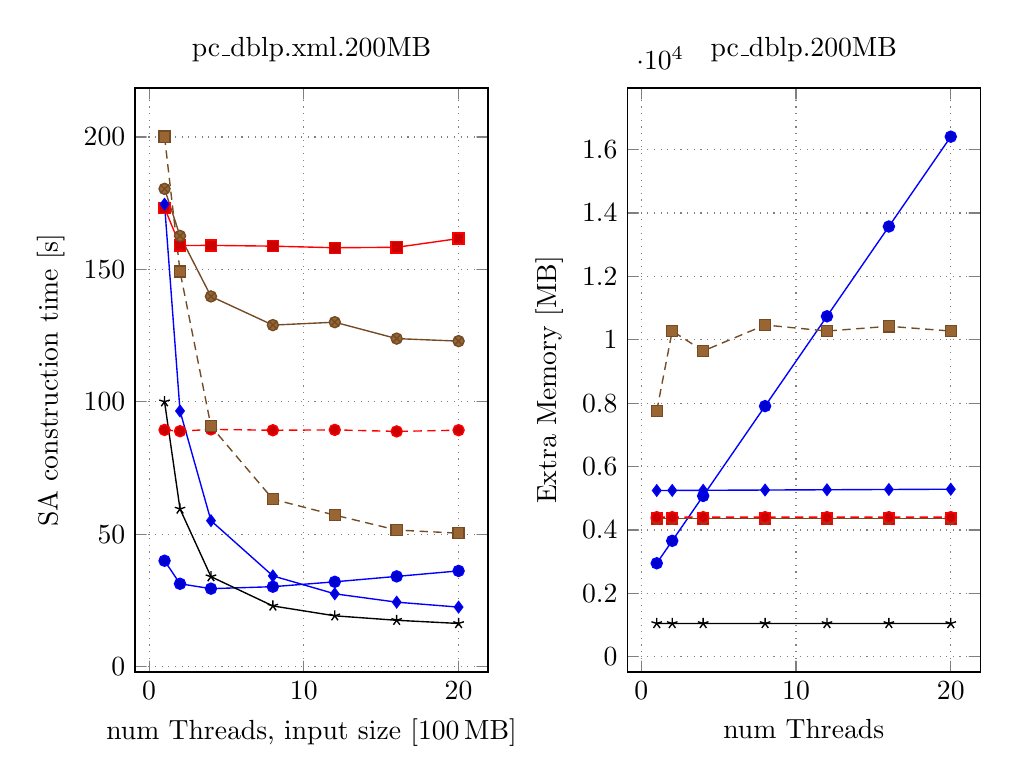
\begin{tikzpicture}
        \begin{axis}[
                name=axis1,
                width=0.5\textwidth,
                height=90mm,
                title={pc\_dblp.xml.200MB},
                xlabel={num Threads, input size [100\,MB]},
                ylabel={SA construction time [s]},
                legend columns=4,
                legend to name=legend1,
                legend style={
                    /tikz/every even column/.append style={column sep=0.5cm,black},
                    /tikz/every even column/.append style={black},
                },
            ]

            %% MULTIPLOT(algo) SELECT thread_count AS x, time/1000 AS y, MULTIPLOT
            %% FROM stats WHERE rep_id=1 AND input="pc_dblp.xml.200MB" GROUP BY MULTIPLOT,x ORDER BY MULTIPLOT,x
            \addplot coordinates { (1,40.0423) (2,31.3452) (4,29.4979) (8,30.2447) (12,32.0876) (16,34.1353) (20,36.2008) };
            \addlegendentry{algo=BPR\_par};
            \addplot coordinates { (1,173.278) (2,159.036) (4,159.092) (8,158.806) (12,158.202) (16,158.372) (20,161.672) };
            \addlegendentry{algo=DC3-Parallel-2};
            \addplot coordinates { (1,180.451) (2,162.678) (4,139.827) (8,129.002) (12,130.097) (16,123.9) (20,122.954) };
            \addlegendentry{algo=DC3\_parallel};
            \addplot coordinates { (1,100.072) (2,59.5914) (4,34.0259) (8,22.9758) (12,19.2516) (16,17.5619) (20,16.3639) };
            \addlegendentry{algo=Deep-Shallow\_par};
            \addplot coordinates { (1,174.646) (2,96.5873) (4,55.1651) (8,34.3187) (12,27.5544) (16,24.406) (20,22.5367) };
            \addlegendentry{algo=Discarding4Parallel};
            \addplot coordinates { (1,89.4281) (2,88.9524) (4,89.6287) (8,89.3064) (12,89.4438) (16,88.8689) (20,89.3215) };
            \addlegendentry{algo=GSACA\_parallel};
            \addplot coordinates { (1,200.129) (2,149.229) (4,90.8389) (8,63.2769) (12,57.2701) (16,51.6274) (20,50.447) };
            \addlegendentry{algo=Osipov\_parallel\_wp};

        \end{axis}
        \begin{axis}[
                at={(axis1.outer north east)},
                anchor=outer north west,
                name=axis2,
                width=0.5\textwidth,
                height=90mm,
                title={pc\_dblp.200MB},
                xlabel={num Threads},
                ylabel={Extra Memory [MB]},
            ]

            %% MULTIPLOT(algo) SELECT thread_count AS x, memPeak/1000000 AS y, MULTIPLOT
            %% FROM (
            %% SELECT algo, input, MEDIAN(memFinal) AS memFinal, MEDIAN(memOff) AS memOff, AVG(memPeak) AS memPeak, prefix, rep, thread_count, MEDIAN(time) AS time FROM stats GROUP BY algo, input, prefix, rep, thread_count
            %% ) WHERE input="pc_dblp.xml.200MB" GROUP BY MULTIPLOT,x ORDER BY MULTIPLOT,x
            \addplot coordinates { (1,2949.79) (2,3658.03) (4,5074.5) (8,7907.44) (12,10740.4) (16,13573.3) (20,16406.3) };
            \addlegendentry{algo=BPR\_par};
            \addplot coordinates { (1,4354.92) (2,4354.92) (4,4354.92) (8,4354.92) (12,4354.92) (16,4354.92) (20,4354.92) };
            \addlegendentry{algo=DC3-Parallel-2};
            \addplot coordinates { (1,4354.92) (2,4354.92) (4,4354.92) (8,4354.92) (12,4354.92) (16,4354.92) (20,4354.92) };
            \addlegendentry{algo=DC3\_parallel};
            \addplot coordinates { (1,1051.11) (2,1051.11) (4,1051.11) (8,1051.11) (12,1051.15) (16,1051.21) (20,1051.27) };
            \addlegendentry{algo=Deep-Shallow\_par};
            \addplot coordinates { (1,5245.03) (2,5247.27) (4,5251.56) (8,5260.14) (12,5268.72) (16,5277.3) (20,5285.88) };
            \addlegendentry{algo=Discarding4Parallel};
            \addplot coordinates { (1,4404.02) (2,4404.02) (4,4404.03) (8,4404.03) (12,4404.04) (16,4404.05) (20,4404.05) };
            \addlegendentry{algo=GSACA\_parallel};
            \addplot coordinates { (1,7759.35) (2,10275.8) (4,9646.71) (8,10465.9) (12,10275.8) (16,10425.2) (20,10275.8) };
            \addlegendentry{algo=Osipov\_parallel\_wp};

            \legend{}
        \end{axis}
    \end{tikzpicture}

    \medskip
    \ref{legend1}
\end{center}

\begin{center}
    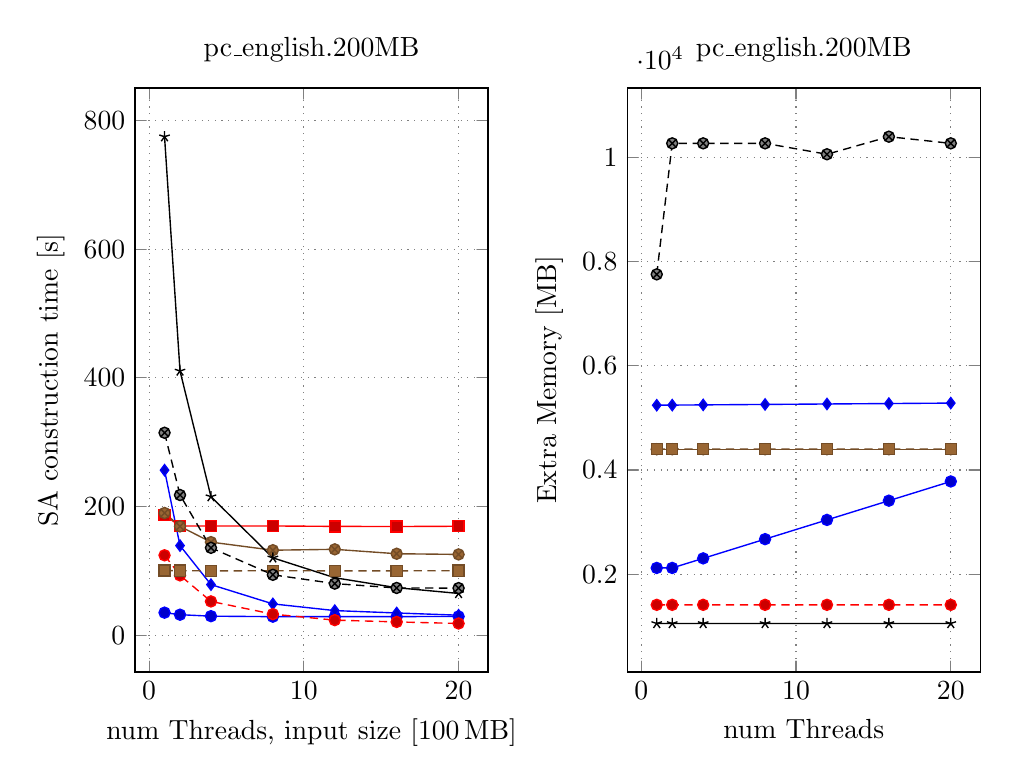
\begin{tikzpicture}
        \begin{axis}[
                name=axis1,
                width=0.5\textwidth,
                height=90mm,
                title={pc\_english.200MB},
                xlabel={num Threads, input size [100\,MB]},
                ylabel={SA construction time [s]},
                legend columns=4,
                legend to name=legend2,
                legend style={
                    /tikz/every even column/.append style={column sep=0.5cm,black},
                    /tikz/every even column/.append style={black},
                },
            ]

            %% MULTIPLOT(algo) SELECT thread_count AS x, time/1000 AS y, MULTIPLOT
            %% FROM stats WHERE rep_id=1 AND input="pc_english.200MB" GROUP BY MULTIPLOT,x ORDER BY MULTIPLOT,x
            \addplot coordinates { (1,35.0036) (2,31.8226) (4,29.523) (8,28.7777) (12,28.8238) (16,28.8382) (20,29.115) };
            \addlegendentry{algo=BPR\_par};
            \addplot coordinates { (1,186.491) (2,169.764) (4,169.663) (8,169.755) (12,169.112) (16,168.919) (20,169.31) };
            \addlegendentry{algo=DC3-Parallel-2};
            \addplot coordinates { (1,189.907) (2,169.171) (4,144.653) (8,132.086) (12,133.452) (16,126.592) (20,125.538) };
            \addlegendentry{algo=DC3\_parallel};
            \addplot coordinates { (1,774.972) (2,410.752) (4,215.338) (8,120.201) (12,89.2563) (16,73.8094) (20,64.8554) };
            \addlegendentry{algo=Deep-Shallow\_par};
            \addplot coordinates { (1,256.556) (2,139.213) (4,78.6018) (8,48.6157) (12,38.2059) (16,34.5034) (20,31.0396) };
            \addlegendentry{algo=Discarding4Parallel};
            \addplot coordinates { (1,124.184) (2,92.9755) (4,52.4646) (8,32.6679) (12,23.3865) (16,20.5833) (20,18.1679) };
            \addlegendentry{algo=DivSufSort\_PARALLEL\_ref};
            \addplot coordinates { (1,100.367) (2,100.275) (4,99.9141) (8,100.174) (12,99.9944) (16,100.009) (20,100.208) };
            \addlegendentry{algo=GSACA\_parallel};
            \addplot coordinates { (1,314.668) (2,217.903) (4,135.771) (8,93.8321) (12,80.1451) (16,73.3822) (20,73.1638) };
            \addlegendentry{algo=Osipov\_parallel\_wp};

        \end{axis}
        \begin{axis}[
                at={(axis1.outer north east)},
                anchor=outer north west,
                name=axis2,
                width=0.5\textwidth,
                height=90mm,
                title={pc\_english.200MB},
                xlabel={num Threads},
                ylabel={Extra Memory [MB]},
            ]

            %% MULTIPLOT(algo) SELECT thread_count AS x, memPeak/1000000 AS y, MULTIPLOT
            %% FROM (
            %% SELECT algo, input, MEDIAN(memFinal) AS memFinal, MEDIAN(memOff) AS memOff, AVG(memPeak) AS memPeak, prefix, rep, thread_count, MEDIAN(time) AS time FROM stats GROUP BY algo, input, prefix, rep, thread_count
            %% ) WHERE input="pc_english.200MB" GROUP BY MULTIPLOT,x ORDER BY MULTIPLOT,x
            \addplot coordinates { (1,2119.12) (2,2119.12) (4,2303) (8,2672.38) (12,3041.77) (16,3411.15) (20,3780.54) };
            \addlegendentry{algo=BPR\_par};
            \addplot coordinates { (1,4399.71) (2,4399.71) (4,4399.71) (8,4399.71) (12,4399.71) (16,4399.71) (20,4399.71) };
            \addlegendentry{algo=DC3-Parallel-2};
            \addplot coordinates { (1,4399.71) (2,4399.71) (4,4399.71) (8,4399.71) (12,4399.71) (16,4399.71) (20,4399.71) };
            \addlegendentry{algo=DC3\_parallel};
            \addplot coordinates { (1,1052.19) (2,1052.19) (4,1052.19) (8,1052.19) (12,1052.33) (16,1052.55) (20,1052.74) };
            \addlegendentry{algo=Deep-Shallow\_par};
            \addplot coordinates { (1,5245.03) (2,5247.27) (4,5251.56) (8,5260.14) (12,5268.72) (16,5277.3) (20,5285.88) };
            \addlegendentry{algo=Discarding4Parallel};
            \addplot coordinates { (1,1410.24) (2,1410.24) (4,1410.25) (8,1410.26) (12,1410.27) (16,1410.28) (20,1410.29) };
            \addlegendentry{algo=DivSufSort\_PARALLEL\_ref};
            \addplot coordinates { (1,4404.02) (2,4404.03) (4,4404.03) (8,4404.04) (12,4404.06) (16,4404.07) (20,4404.08) };
            \addlegendentry{algo=GSACA\_parallel};
            \addplot coordinates { (1,7759.38) (2,10275.9) (4,10275.9) (8,10275.9) (12,10066.2) (16,10403.7) (20,10275.9) };
            \addlegendentry{algo=Osipov\_parallel\_wp};

            \legend{}
        \end{axis}
    \end{tikzpicture}

    \medskip
    \ref{legend2}
\end{center}

\begin{center}
    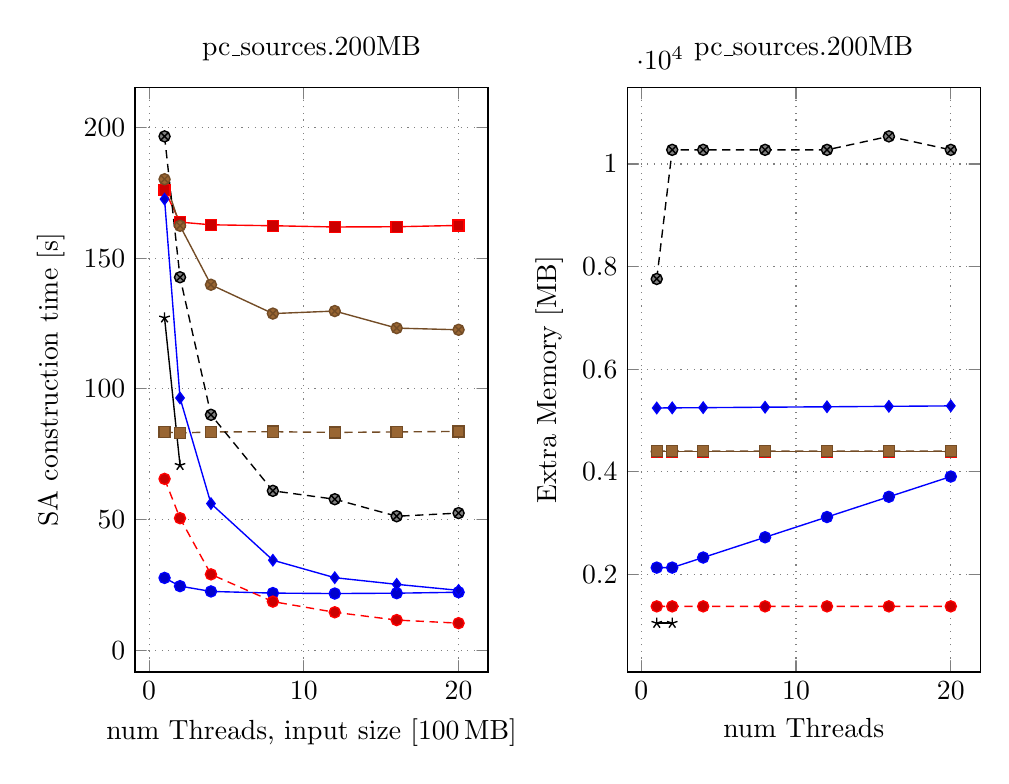
\begin{tikzpicture}
        \begin{axis}[
                name=axis1,
                width=0.5\textwidth,
                height=90mm,
                title={pc\_sources.200MB},
                xlabel={num Threads, input size [100\,MB]},
                ylabel={SA construction time [s]},
                legend columns=4,
                legend to name=legend4,
                legend style={
                    /tikz/every even column/.append style={column sep=0.5cm,black},
                    /tikz/every even column/.append style={black},
                },
            ]

            %% MULTIPLOT(algo) SELECT thread_count AS x, time/1000 AS y, MULTIPLOT
            %% FROM stats WHERE rep_id=1 AND input="pc_sources.200MB" GROUP BY MULTIPLOT,x ORDER BY MULTIPLOT,x
            \addplot coordinates { (1,27.6434) (2,24.4874) (4,22.4577) (8,21.8211) (12,21.6541) (16,21.7886) (20,22.1477) };
            \addlegendentry{algo=BPR\_par};
            \addplot coordinates { (1,176.134) (2,163.88) (4,162.846) (8,162.492) (12,162.014) (16,162.103) (20,162.612) };
            \addlegendentry{algo=DC3-Parallel-2};
            \addplot coordinates { (1,180.301) (2,162.476) (4,139.896) (8,128.855) (12,129.819) (16,123.293) (20,122.649) };
            \addlegendentry{algo=DC3\_parallel};
            \addplot coordinates { (1,127.236) (2,70.7708) };
            \addlegendentry{algo=Deep-Shallow\_par};
            \addplot coordinates { (1,172.696) (2,96.5509) (4,56.1017) (8,34.4222) (12,27.7215) (16,25.1809) (20,22.8794) };
            \addlegendentry{algo=Discarding4Parallel};
            \addplot coordinates { (1,65.5605) (2,50.5047) (4,28.9966) (8,18.5655) (12,14.4738) (16,11.4979) (20,10.313) };
            \addlegendentry{algo=DivSufSort\_PARALLEL\_ref};
            \addplot coordinates { (1,83.5018) (2,83.1187) (4,83.5395) (8,83.6168) (12,83.3511) (16,83.5401) (20,83.73) };
            \addlegendentry{algo=GSACA\_parallel};
            \addplot coordinates { (1,196.706) (2,142.763) (4,90.0987) (8,60.9789) (12,57.7707) (16,51.2473) (20,52.4599) };
            \addlegendentry{algo=Osipov\_parallel\_wp};

        \end{axis}
        \begin{axis}[
                at={(axis1.outer north east)},
                anchor=outer north west,
                name=axis2,
                width=0.5\textwidth,
                height=90mm,
                title={pc\_sources.200MB},
                xlabel={num Threads},
                ylabel={Extra Memory [MB]},
            ]

            %% MULTIPLOT(algo) SELECT thread_count AS x, memPeak/1000000 AS y, MULTIPLOT
            %% FROM (
            %% SELECT algo, input, MEDIAN(memFinal) AS memFinal, MEDIAN(memOff) AS memOff, AVG(memPeak) AS memPeak, prefix, rep, thread_count, MEDIAN(time) AS time FROM stats GROUP BY algo, input, prefix, rep, thread_count
            %% ) WHERE input="pc_sources.200MB" GROUP BY MULTIPLOT,x ORDER BY MULTIPLOT,x
            \addplot coordinates { (1,2134.82) (2,2134.82) (4,2331.19) (8,2725.64) (12,3120.09) (16,3514.53) (20,3908.98) };
            \addlegendentry{algo=BPR\_par};
            \addplot coordinates { (1,4397.55) (2,4397.55) (4,4397.55) (8,4397.55) (12,4397.55) (16,4397.55) (20,4397.55) };
            \addlegendentry{algo=DC3-Parallel-2};
            \addplot coordinates { (1,4397.55) (2,4397.55) (4,4397.55) (8,4397.55) (12,4397.55) (16,4397.55) (20,4397.55) };
            \addlegendentry{algo=DC3\_parallel};
            \addplot coordinates { (1,1052.25) (2,1052.25) };
            \addlegendentry{algo=Deep-Shallow\_par};
            \addplot coordinates { (1,5245.03) (2,5247.27) (4,5251.56) (8,5260.14) (12,5268.72) (16,5277.3) (20,5285.88) };
            \addlegendentry{algo=Discarding4Parallel};
            \addplot coordinates { (1,1379.09) (2,1379.09) (4,1379.09) (8,1379.1) (12,1379.1) (16,1379.12) (20,1379.12) };
            \addlegendentry{algo=DivSufSort\_PARALLEL\_ref};
            \addplot coordinates { (1,4404.02) (2,4404.03) (4,4404.03) (8,4404.05) (12,4404.06) (16,4404.07) (20,4404.08) };
            \addlegendentry{algo=GSACA\_parallel};
            \addplot coordinates { (1,7759.28) (2,10275.7) (4,10275.7) (8,10275.7) (12,10275.7) (16,10538) (20,10275.7) };
            \addlegendentry{algo=Osipov\_parallel\_wp};

            \legend{}
        \end{axis}
    \end{tikzpicture}

    \medskip
    \ref{legend3}
\end{center}

\begin{center}
    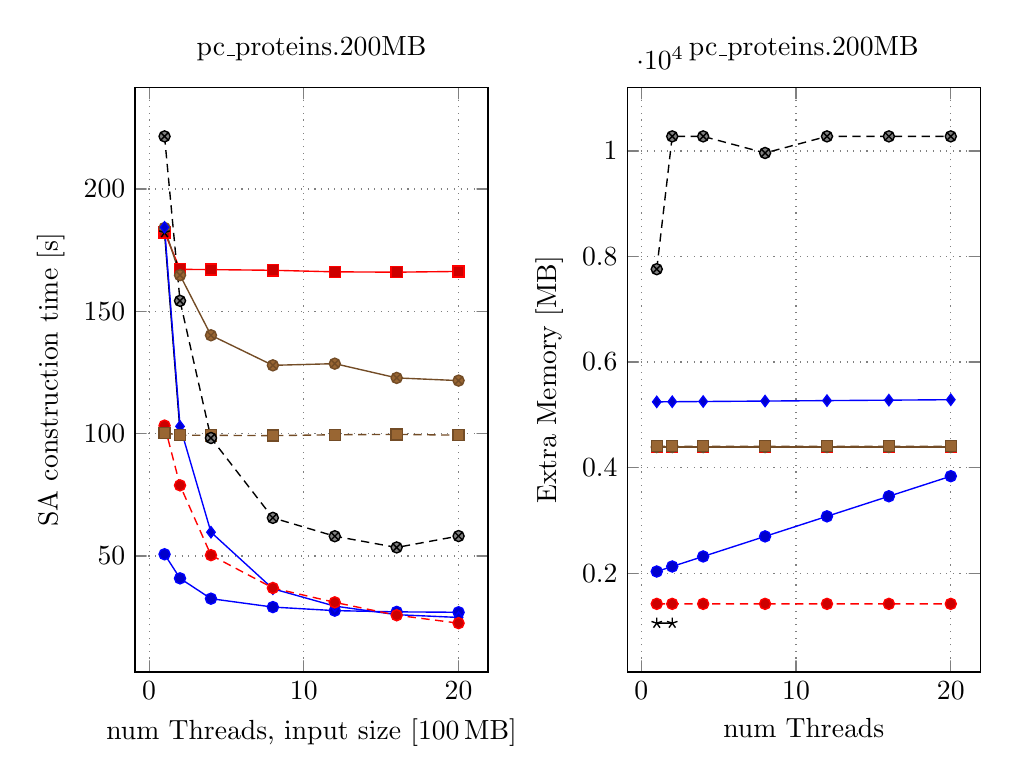
\begin{tikzpicture}
        \begin{axis}[
                name=axis1,
                width=0.5\textwidth,
                height=90mm,
                title={pc\_proteins.200MB},
                xlabel={num Threads, input size [100\,MB]},
                ylabel={SA construction time [s]},
                legend columns=4,
                legend to name=legend3,
                legend style={
                    /tikz/every even column/.append style={column sep=0.5cm,black},
                    /tikz/every even column/.append style={black},
                },
            ]

            %% MULTIPLOT(algo) SELECT thread_count AS x, time/1000 AS y, MULTIPLOT
            %% FROM stats WHERE rep_id=1 AND input="pc_proteins.200MB" GROUP BY MULTIPLOT,x ORDER BY MULTIPLOT,x
            \addplot coordinates { (1,50.7243) (2,40.8852) (4,32.5718) (8,29.1395) (12,27.691) (16,27.1841) (20,27.0186) };
            \addlegendentry{algo=BPR\_par};
            \addplot coordinates { (1,182.26) (2,167.169) (4,167.048) (8,166.777) (12,166.14) (16,166.004) (20,166.306) };
            \addlegendentry{algo=DC3-Parallel-2};
            \addplot coordinates { (1,184.08) (2,164.782) (4,140.219) (8,127.934) (12,128.618) (16,122.798) (20,121.694) };
            \addlegendentry{algo=DC3\_parallel};
            \addplot coordinates { (1,182.174) (2,100.927) };
            \addlegendentry{algo=Deep-Shallow\_par};
            \addplot coordinates { (1,184.336) (2,102.986) (4,59.7464) (8,36.6262) (12,29.5335) (16,26.0342) (20,24.9066) };
            \addlegendentry{algo=Discarding4Parallel};
            \addplot coordinates { (1,103.308) (2,78.8908) (4,50.3562) (8,36.9487) (12,31.0736) (16,25.8079) (20,22.5701) };
            \addlegendentry{algo=DivSufSort\_PARALLEL\_ref};
            \addplot coordinates { (1,100.368) (2,99.3524) (4,99.3332) (8,99.1998) (12,99.5623) (16,99.7004) (20,99.401) };
            \addlegendentry{algo=GSACA\_parallel};
            \addplot coordinates { (1,221.497) (2,154.296) (4,98.2361) (8,65.6032) (12,58.0968) (16,53.5098) (20,58.1636) };
            \addlegendentry{algo=Osipov\_parallel\_wp};

        \end{axis}
        \begin{axis}[
                at={(axis1.outer north east)},
                anchor=outer north west,
                name=axis2,
                width=0.5\textwidth,
                height=90mm,
                title={pc\_proteins.200MB},
                xlabel={num Threads},
                ylabel={Extra Memory [MB]},
            ]

            %% MULTIPLOT(algo) SELECT thread_count AS x, memPeak/1000000 AS y, MULTIPLOT
            %% FROM (
            %% SELECT algo, input, MEDIAN(memFinal) AS memFinal, MEDIAN(memOff) AS memOff, AVG(memPeak) AS memPeak, prefix, rep, thread_count, MEDIAN(time) AS time FROM stats GROUP BY algo, input, prefix, rep, thread_count
            %% ) WHERE input="pc_proteins.200MB" GROUP BY MULTIPLOT,x ORDER BY MULTIPLOT,x
            \addplot coordinates { (1,2030.02) (2,2125.07) (4,2315.17) (8,2695.38) (12,3075.59) (16,3455.79) (20,3836) };
            \addlegendentry{algo=BPR\_par};
            \addplot coordinates { (1,4389.47) (2,4389.47) (4,4389.47) (8,4389.47) (12,4389.47) (16,4389.47) (20,4389.47) };
            \addlegendentry{algo=DC3-Parallel-2};
            \addplot coordinates { (1,4389.47) (2,4389.47) (4,4389.47) (8,4389.47) (12,4389.47) (16,4389.47) (20,4389.47) };
            \addlegendentry{algo=DC3\_parallel};
            \addplot coordinates { (1,1050.94) (2,1051.5) };
            \addlegendentry{algo=Deep-Shallow\_par};
            \addplot coordinates { (1,5245.03) (2,5247.27) (4,5251.56) (8,5260.14) (12,5268.72) (16,5277.3) (20,5285.88) };
            \addlegendentry{algo=Discarding4Parallel};
            \addplot coordinates { (1,1416.84) (2,1416.84) (4,1416.84) (8,1416.86) (12,1416.86) (16,1416.85) (20,1416.88) };
            \addlegendentry{algo=DivSufSort\_PARALLEL\_ref};
            \addplot coordinates { (1,4404.02) (2,4404.02) (4,4404.02) (8,4404.03) (12,4404.03) (16,4404.04) (20,4404.04) };
            \addlegendentry{algo=GSACA\_parallel};
            \addplot coordinates { (1,7759.46) (2,10276) (4,10276) (8,9961.48) (12,10276.1) (16,10276.1) (20,10276.1) };
            \addlegendentry{algo=Osipov\_parallel\_wp};

            \legend{}
        \end{axis}
    \end{tikzpicture}

    \medskip
    \ref{legend3}
\end{center}

%\section{Example: 4 plots aligned}
%\begin{center}
%    \begin{tikzpicture}
%        \begin{axis}[
%                name=axis1,
%                width=0.5\textwidth,
%                height=70mm,
%                title={pc\_english.200MB},
%                xlabel={File size [MB]},
%                ylabel={SA construction time [s]},
%            ]
%
%            %% MULTIPLOT(algo) SELECT prefix/1000000 AS x, time AS y, MULTIPLOT
%            %% FROM stats WHERE algo="BPR_dummy" GROUP BY MULTIPLOT,x ORDER BY MULTIPLOT,x
%            \addplot coordinates { (10,1234.0) (20,2954.0) (30,4649.0) (40,6433.0) (50,8303.0) (60,10145.0) (70,12131.0) (80,13990.0) (90,16116.0) (100,18045.0) (110,21886.0) (120,22299.0) (130,24388.0) (140,26642.0) (150,28733.0) (160,30743.0) (170,33016.0) (180,35528.0) (190,37823.0) (200,40068.0) };
%            \addlegendentry{algo=BPR\_dummy};
%
%        \end{axis}
%        \begin{axis}[
%                at={(axis1.outer north east)},
%                anchor=outer north west,
%                name=axis2,
%                width=0.5\textwidth,
%                height=70mm,
%                title={pc\_english.200MB},
%                xlabel={File size [MB]},
%            ]
%
%            %% MULTIPLOT(algo) SELECT prefix/1000000 AS x, time AS y, MULTIPLOT
%            %% FROM stats WHERE algo="BPR_dummy" GROUP BY MULTIPLOT,x ORDER BY MULTIPLOT,x
%            \addplot coordinates { (10,1234.0) (20,2954.0) (30,4649.0) (40,6433.0) (50,8303.0) (60,10145.0) (70,12131.0) (80,13990.0) (90,16116.0) (100,18045.0) (110,21886.0) (120,22299.0) (130,24388.0) (140,26642.0) (150,28733.0) (160,30743.0) (170,33016.0) (180,35528.0) (190,37823.0) (200,40068.0) };
%            \addlegendentry{algo=BPR\_dummy};
%
%        \end{axis}
%        \begin{axis}[
%                at={(axis1.outer south west)},
%                anchor=outer north west,
%                name=axis3,
%                width=0.5\textwidth,
%                height=70mm,
%                title={pc\_english.200MB},
%                xlabel={File size [MB]},
%                ylabel={SA construction time [s]},
%            ]
%
%            %% MULTIPLOT(algo) SELECT prefix/1000000 AS x, time AS y, MULTIPLOT
%            %% FROM stats WHERE algo="BPR_dummy" GROUP BY MULTIPLOT,x ORDER BY MULTIPLOT,x
%            \addplot coordinates { (10,1234.0) (20,2954.0) (30,4649.0) (40,6433.0) (50,8303.0) (60,10145.0) (70,12131.0) (80,13990.0) (90,16116.0) (100,18045.0) (110,21886.0) (120,22299.0) (130,24388.0) (140,26642.0) (150,28733.0) (160,30743.0) (170,33016.0) (180,35528.0) (190,37823.0) (200,40068.0) };
%            \addlegendentry{algo=BPR\_dummy};
%
%        \end{axis}
%        \begin{axis}[
%                at={(axis3.outer north east)},
%                anchor=outer north west,
%                name=axis4,
%                width=0.5\textwidth,
%                height=70mm,
%                title={pc\_english.200MB},
%                xlabel={File size [MB]},
%            ]
%
%            %% MULTIPLOT(algo) SELECT prefix/1000000 AS x, time AS y, MULTIPLOT
%            %% FROM stats WHERE algo="BPR_dummy" GROUP BY MULTIPLOT,x ORDER BY MULTIPLOT,x
%            \addplot coordinates { (10,1234.0) (20,2954.0) (30,4649.0) (40,6433.0) (50,8303.0) (60,10145.0) (70,12131.0) (80,13990.0) (90,16116.0) (100,18045.0) (110,21886.0) (120,22299.0) (130,24388.0) (140,26642.0) (150,28733.0) (160,30743.0) (170,33016.0) (180,35528.0) (190,37823.0) (200,40068.0) };
%            \addlegendentry{algo=BPR\_dummy};
%
%        \end{axis}
%    \end{tikzpicture}
%\end{center}
%
%\section{Extra memory usage}
%\begin{center}
%    \begin{tikzpicture}
%        \begin{axis}[
%                title={pc\_english.200MB},
%                xlabel={File Size [Bytes]},
%                ylabel={Extra Memory [Bytes]},
%            ]
%
%            %% MULTIPLOT(algo) SELECT prefix AS x, memPeak AS y, MULTIPLOT
%            %% FROM stats WHERE algo="BPR_dummy" GROUP BY MULTIPLOT,x ORDER BY MULTIPLOT,x
%            \addplot coordinates { (10000000,10000000) (1e+08,1e+08) (1.1e+08,1.1e+08) (1.2e+08,1.2e+08) (1.3e+08,1.3e+08) (1.4e+08,1.4e+08) (1.5e+08,1.5e+08) (1.6e+08,1.6e+08) (1.7e+08,1.7e+08) (1.8e+08,1.8e+08) (1.9e+08,1.9e+08) (20000000,20000000) (2e+08,2e+08) (30000000,30000000) (40000000,40000000) (50000000,50000000) (60000000,60000000) (70000000,70000000) (80000000,80000000) (90000000,90000000) };
%            \addlegendentry{algo=BPR\_dummy};
%
%        \end{axis}
%    \end{tikzpicture}
%\end{center}
%
%\section{Extra memory per input byte}
%\begin{center}
%    \begin{tikzpicture}
%        \begin{axis}[
%                title={pc\_english.200MB},
%                xlabel={File Size [MB]},
%                ylabel={Extra Memory in Bytes per input Byte},
%            ]
%
%            %% MULTIPLOT(algo) SELECT prefix/1000000 AS x, memPeak/prefix AS y, MULTIPLOT
%            %% FROM stats WHERE algo="BPR_dummy" GROUP BY MULTIPLOT,x ORDER BY MULTIPLOT,x
%            \addplot coordinates { (10,1) (20,1) (30,1) (40,1) (50,1) (60,1) (70,1) (80,1) (90,1) (100,1) (110,1) (120,1) (130,1) (140,1) (150,1) (160,1) (170,1) (180,1) (190,1) (200,1) };
%            \addlegendentry{algo=BPR\_dummy};
%
%        \end{axis}
%    \end{tikzpicture}
%\end{center}
%
\end{document}
